\documentclass[../main.tex]{subfiles}
\graphicspath{{\subfix{../images/}}}

\begin{document}

\section{Τελική σύνδεση}
Τέλος για να συνδεθούν όλα τα modules μαζί φτιάχτηκε ένα νέο module
\textit{MyModule} το οποίο κάνει τις απαραίτητες συνδέσεις. Το \textit{MyModule}
έχει ως εισόδους τα 7 bits data, 1 bit write και noise και ως εξόδους τις 4
ανόδους και τα 6 led. Το \textit{MyModule} ήταν απαραίτητο ώστε να το yosys να
θεωρήσει όλα τα άλλα modules ως blackbox.

\begin{figure}[H]
  \begin{center}
    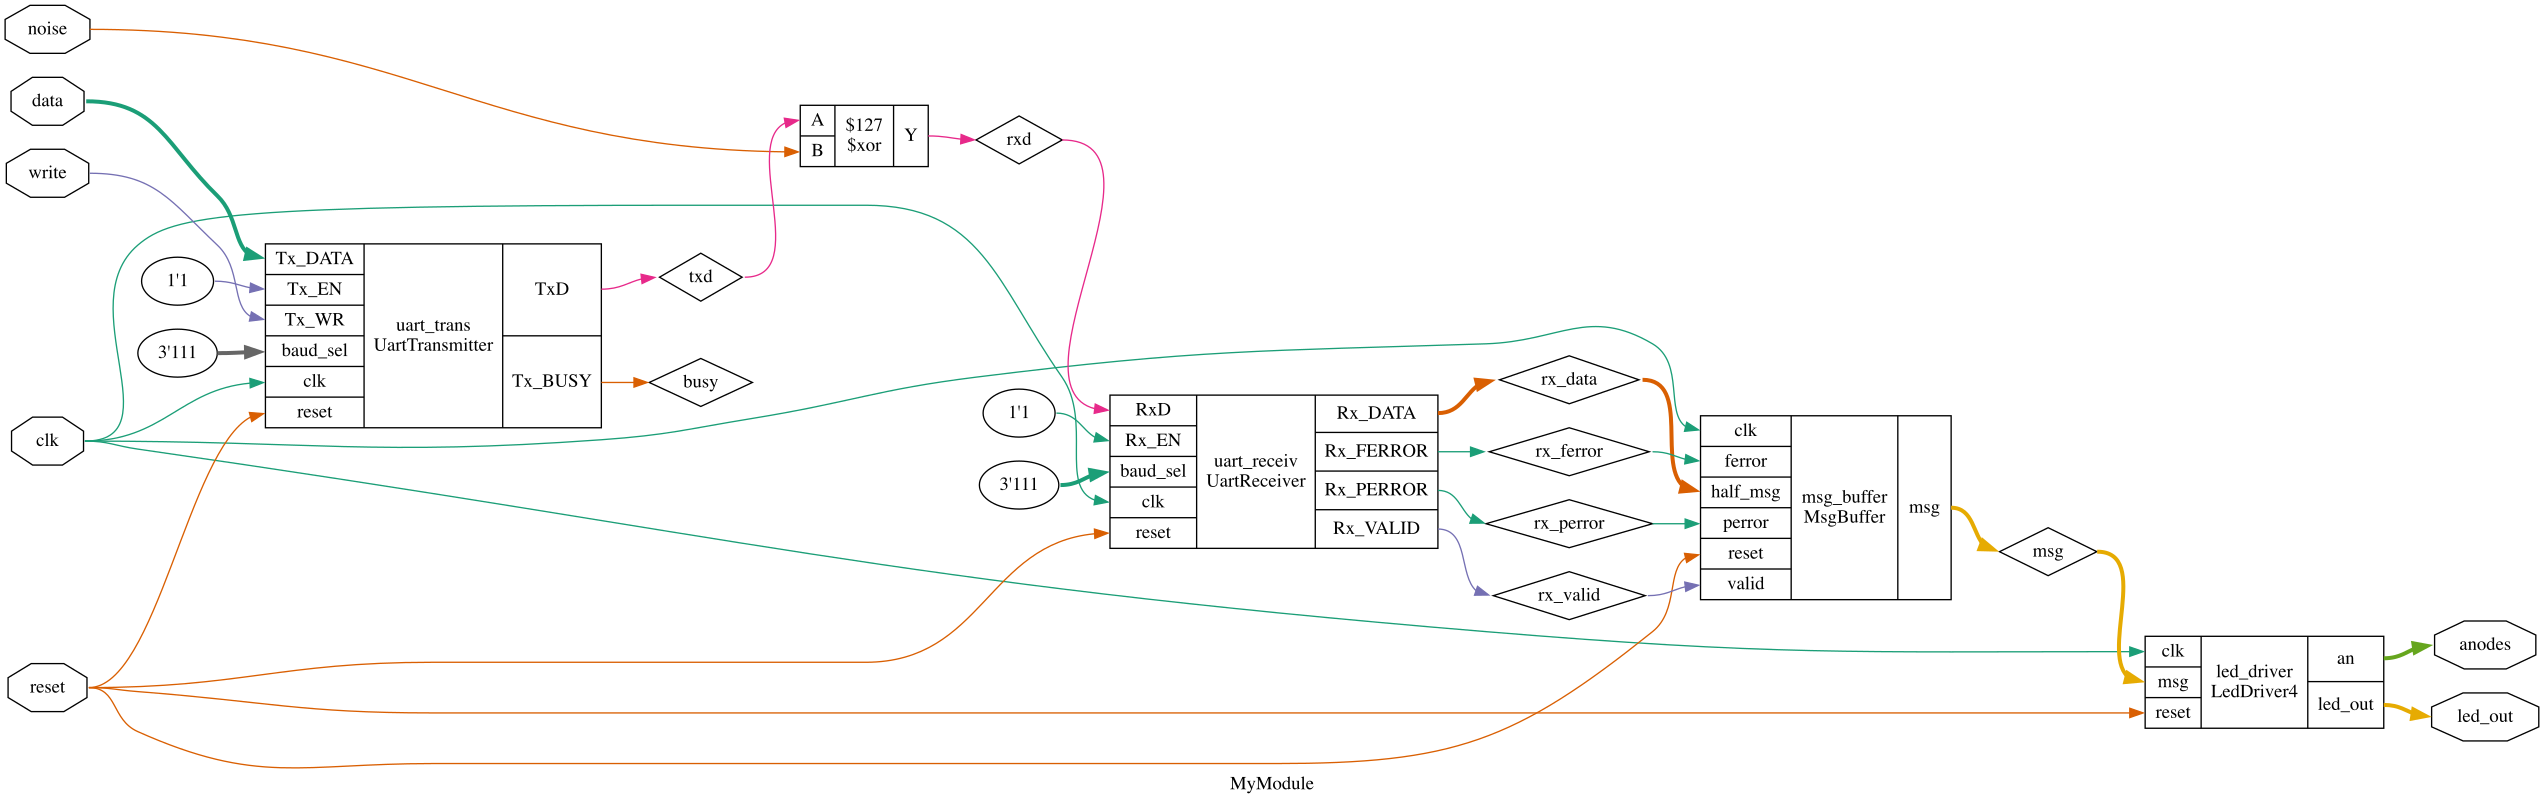
\includegraphics[width=\textwidth]{../../diagrams/MyModule.png}
  \end{center}
  \caption{Τελική συνδεσμολογία όλων των modules.}
  \label{fig:final}
\end{figure}

Όπως φαίνεται στο Σχήμα~\ref{fig:final} το noise περνάει μέσα από μια XOR μαζί
με το TxD και παράγουν το RxD ώστε θέτοντας το noise σε '1' να αντιστρέφουμε το
σήμα που λαμβάνει ο δέκτης και έτσι να προσομοιάσουμε θόρυβο.

Επίσης ανάμεσα από το \textit{UartReceiver} και \textit{LedDriver4} υπάρχει άλλο
ένα module το οποίο ήταν απαραίτητο για την ολοκλήρωση της εργασίας. Επειδή το
μήνυμα που θέλουμε να δείξουμε στην οθόνη είναι 16 bits αλλά ο αποστολέας κι ο
δέκτης επικοινωνούν 8 bits την φορά αυτό σημαίνει ότι θα χρειαστούμε 2 λήψεις
ώστε να έχουμε ένα πλήρες μήνυμα. Το \textit{MsgBuffer} module λοιπόν αυτό που
κάνει είναι να εξάγει 16 bits msg μετά από 2 valid half\_msg που έχει λάβει από
τον UartReceiver και αν εντοπίσει είτε perror είτε ferror κάνει το msg 'FFFF'.

\begin{figure}[H]
  \begin{center}
    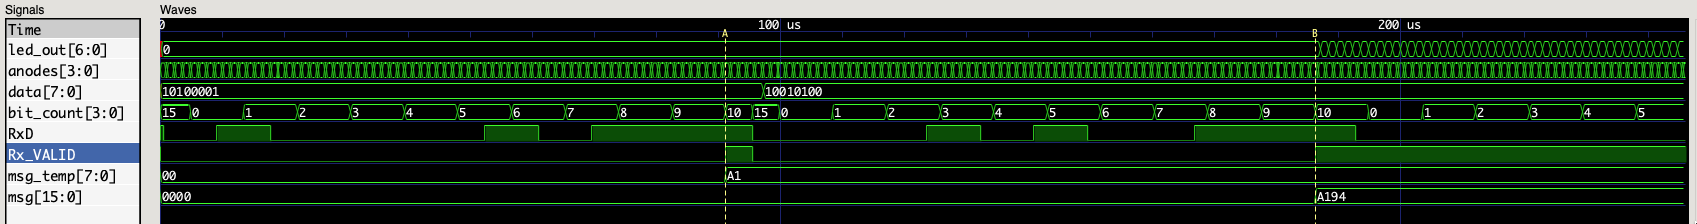
\includegraphics[width=\textwidth]{../images/mymodule_tb.png}
  \end{center}
  \caption{Αποστολή '-194' και εμφάνιση στις οθόνες.}
  \label{fig:final_-194}
\end{figure}

Στο Σχήμα~\ref{fig:final_-194} την χρονική στιγμή A φτάνει το τελευταίο bit του
πρώτου μηνύματος και το μήνυμα υπολογίζεται ως valid. Εκείνη την στιγμή το 8
bits μήνυμα αποθηκεύεται στο msg\_tmp register του \textit{MsgBuffer}. Την
χρονική στιγμή B φτάνει 2\textsuperscript{ο} VALID μήνυμα και τότε το
\textit{MsgBuffer} το ενώνει με το άλλο μισό που έλαβε προηγουμένως και το
περνάει στο \textit{LedDriver4}.

Μεγεθύνοντας στην χρονική περίοδο B και μετά, δηλαδή αφού έχει ληφθεί το πλήρες
μήνυμα (Σχήμα~\ref{fig:final_ledout}), βλέπουμε ότι τιμή του led\_out είναι
σωστή την κατάλληλη χρονική στιγμή. Δηλαδή την στιγμή που η άνοδος 3 είναι στο 0
στο led\_out έχουμε τιμή '-' άρα στην πρώτη οθόνη θα εμφανιστεί ο χαρακτήρας
'-', αντίστοιχα και για τις άλλες ανόδους, έτσι καταλαβαίνουμε ότι το μήνυμα που
θα δούμε στις 4 οθόνες είναι '-194'.

\begin{figure}[H]
  \begin{center}
    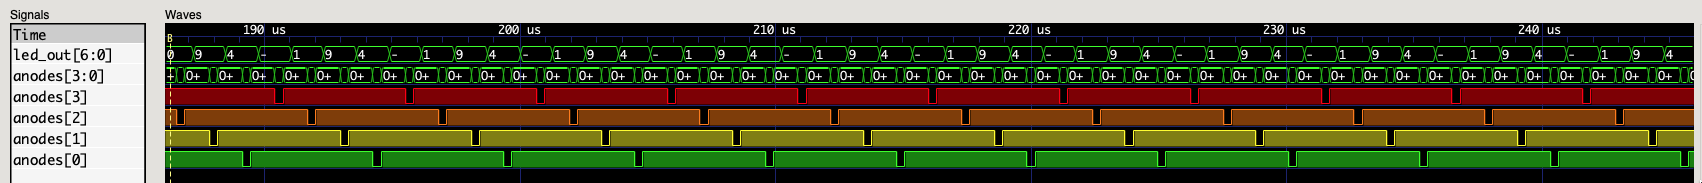
\includegraphics[width=\textwidth]{../images/mymodule_ledout.png}
  \end{center}
  \caption{Αποστολή '-194' και εμφάνιση στις οθόνες αφού έχει ληφθεί το πλήρες
  μήνυμα.}
  \label{fig:final_ledout}
\end{figure}

Τέλος στο Σχήμα~\ref{fig:final_parity_error} βλέπου την περίπτωση όπου το
\textit{MsgBuffer} εντοπίζει parity error από το πρώτο κιόλας πακέτο άρα κάνει
την έξοδό του msg 'FFFF'.

\begin{figure}[H]
  \begin{center}
    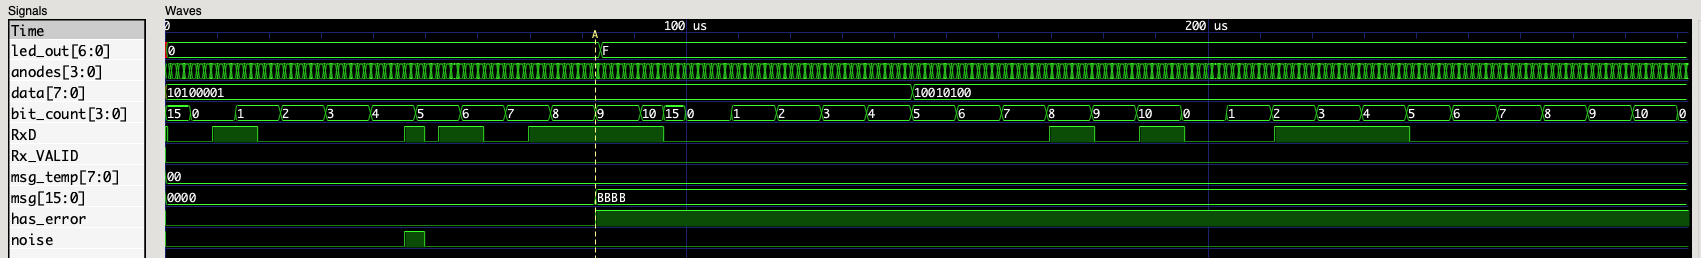
\includegraphics[width=\textwidth]{../images/final_parity_error.png}
  \end{center}
  \caption{Αποστολή '-194' με parity error.}
  \label{fig:final_parity_error}
\end{figure}

\end{document}
